\subsection{Parallelisierung}
Zur Parallelisierung des Merge-Sort Algorithmus wird aufgrund beschränkter Zeit ein vereinfachter Algorithmus verwendet.\\
Die zu sortierenden Daten werden auf der Master Knoten in Datenblöcke gleicher Wörterzahl gespaltet. Verwendet wird der standard template library Datentyp \textit{std::vector} (im Folgenden: Vektor). Die Anzahl der Vektoren entspricht der Anzahl der verfügbaren Rechenknoten (Slave Knoten). Der Datensatz wird unsortiert möglichst gleich auf die Vektoren verteilt. Eine Konvertierung von einem Vektor von Zeichenketten (\textit{std::string}) in ein einzelnes, großes \textit{char}-Array unter Verwendung von Trennzeichen ermöglicht die Übertragung des Datensatzes, welcher für den jeweiligen Slave-Knoten bestimmt ist, in einer einzigen Nachricht. 
\\
Auf den Slave-Knoten werden die Char-Arrays wieder in Vektoren von Zeichenketten umgewandelt, was die Verwendung der bestehenden Implementierung des Merge-Sort Algorithmus erleichtert. Mittels Merge Sort werden die Elemente des Vektors sortiert. Der sortierte Vektor wird erneut über Umwandlung in ein Char-Array zurück zur Master Node geschickt. Auf dem Master Knoten werden nach Erhalt der Ergebnisse aller Slave Knoten diese in einer \textit{double-ended queue}(im Folgenden: deque) aus Vektoren gespeichert, mit der Funktion \texit{merge\_back()} zusammengeführt und als Ergebnis ausgegeben. In  \texit{merge\_back()} werden jeweils die ersten beiden Vektoren aus der deque entfernt und mit der bestehenden Funktion \textit{merge} zusammengeführt. Daraus wird erneut ein Vektor gebildet, welcher an das Ende des deque angehängt wird. Dieser Algorithmus wird ausgeführt bis die Anzahl der Elemente in der deque auf eins reduziert ist. Der einzig verbleibende Vektor in der deque wird als Endergebnis ausgegeben und beinhaltet die sortierten Daten. 
\\
\begin{figure}[!t]
	\centering
	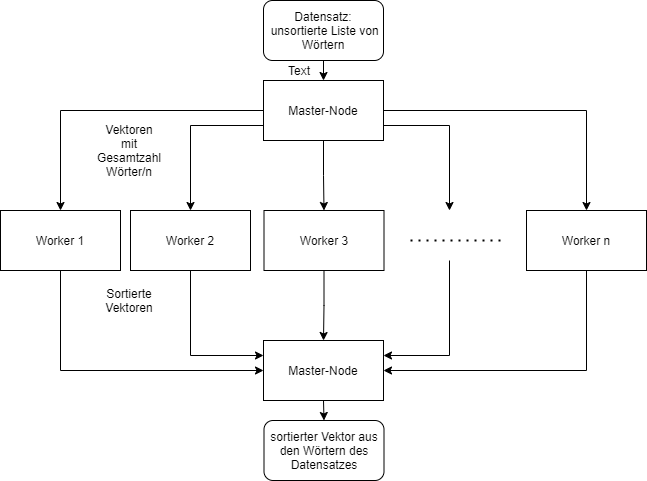
\includegraphics[width=3.5in]{Parallelisierungs_Algorithmus.png}
	\caption{Datenfluss des implementierten Algorithmus}
	\label{para_algo1}
\end{figure}
Basierend auf der Aufteilung kann eine beliebige natürliche Zahl an Rechenknoten verwendet werden. Die Sortierung der Teil-Vektoren wird hierbei immer von allen Nodes ausschließlich dem Master übernommen.

